\section*{Introduction}
\begin{frame}{Deep Learning Lab: Welcome}
\textbf{Structure and objectives:}
  \begin{itemize}
\item Acquire hands-on experience - \textit{Lab}!
\item Focus on practical aspects of machine learning/deep learning\\
($\approx$ 50\% lectures, 50\% exercises)
\item (Originally designed to) Complement the lecture \textit{Machine Learning}
\item But self-contained.
% \item Otherwise designed for broad audience.
\end{itemize}

\vspace{5mm}
\textbf{Introduction to:}
\begin{itemize}
\item Framework, tools, implementation (PyTorch)
\item Basic \textbf{practicalities} of deep learning:
workflow, hyper-parameter tuning, practical tricks...
\item ...using various types of problems and model architectures
\item Learning to autonomously search for knowledge/solution to problems
\end{itemize}

%Share our knowledge based on experiences in coding, tuning, problem solving...\\
%Many of what we will tell are recommendations, suggestions.\\
%Practice has no absolutely right answers/approach.
%In the end of this lecture, we would like you to be able to...
\end{frame}

% Schedule 2019:
% Topic 1: 1 - 19. (20/09) + Act 1. # intro: applications, python, virtualenv, numpy, colab, TF.
% Topic 2: 20 - 30. (27/09) + Act 2.  # TF basics.
% Topic 3: 31 - 38. (04/10 and 11/10) + Act 3 # Start: fundamental models, linear regression. 
% Topic 4: 39 - 49. (18/10) + Act 4  # classification, FFNN, MNIST.
% Topic 5: 50 - 60. (25/10) + Act 5  # CNN, MNIST again.
% Topic 6: 61 - 74. (08/11) + Act 6  # RNN, n-back.
% Topic 7: 75 - 85. (15/11 and 22/11) + Act 7  # LSTM, n-back again.
% Topic 8: 86 - 98. (29/11, 06/12, 13/12, 20/12)  # selected models + RL?
% Act 8 distributed on 06/12.

% i.e. Act 3 and 7 takes the whole day. + Act 8 multiple days?

% Schedule 2020:
% Room A21.
% 14 days.
% Tentative plan: 7 1/2 days exercises + 6 1/2 days lectures?
% 01 - 13. (18/09): Intro + Act 1 (Python basics).
% (25/09): [Change order? introduce PyTorch basics first??] + Act 2 (PyTorch basics?)
% (02/10): workflow overview
% Topic 3:  (02/10 and 9/10)
% (9/10): 
% Topic 4:  (16/10)
% Topic 5:  (23/10)
% Topic 6:  (30/10)
% Topic 7:  (06/11 and 13/11)
% Topic 8:  (20/11, 27/11, 4/12, 11/12, 18/12)

% ===================
%  Lecture contents:
% ===================
% Intro (half) 1 - 13++
% Workflow (full day) 14 - 30
% PyTorch  basics (full) Tensor manipulation + Auto diff. 31 - 62
% Implementation of systems, whole pipeline, FF model, MNIST. 63 - 85 --> E4.
% Start: fundamental blocks: CNN. 86 - 100. --> E5/A2.

% RNN, residual connections. 101 - 109.
% Attention, self-attention, Transformers: 110 - 121.
% Start: Practical tricks.  122 - 135.
% Start: Building models. encoder-decoder 136 - 146
% enc-dec + attention: 147 - 154.
% Summary & final words: 155 - 165.

% ===================
%  Exercises:
% ===================
% E1: Intro to Python, Colab etc. (half?)
% E2: Intro to PyTorch?? Basic Tensor manipulation? (full?)
% E3/A1: First PyTorch applied exercise? regression? (full?)
% E4: MNIST FF model + extra (half? make it full?)
% E5/A2: CNN CIFAR (full?)
% E6: RNN basics (half?)
% E7/A3: Language modeling (RNN + Trafo?) (full)
% E8/A4: Final deepmind math. (full or more?)


% Put assignments one week before the dedicated session,
% leave them 2 weeks after the session to finish.
% (total 3 weeks.)

% Tentative plan:
% (18/09): Intro + E1 (Python basics).
% (25/09): Workflow (full day) 14 - 30, + PyTorch basics?
% (02/10): PyTorch  more example, regression + E2.
% (9/10): E3/A1.

% (16/10): Implementation of systems, whole pipeline, FF model, MNIST. 63 - 85 --> E4.
% (23/10): Start: fundamental blocks: CNN. 86 - 100. --> distribute E5/A2.
% (30/10): E5/A2.

% (06/11): RNN, residual connections. 101 - 109. + E6
% (13/11): Attention, self-attention, Transformers: 110 - 121. no exercise.
% (20/11): E7/A3.

% (27/11): Practical tricks.  122 - 135. no exercise?
% (4/12): Building models. encoder-decoder 136 - 146 + attn 147 - 154. --> distribute E8/A4.
% (11/12): E8/A4.

% (18/12): Summary & final words: 155 - 165.

\begin{frame}{Course Logistics}
%\vspace{-3mm}
\textbf{Time and location:}
\begin{itemize}
\item \textbf{Mondays from 10:30 to 12:00} (no break in principle)
\item Lecture room: \textbf{C1.03} Est Campus \link{https://www.desk.usi.ch/en/lugano-campus-map-access-facilities}
\end{itemize}
\pause
\vsp
\textbf{Format:}
  \begin{itemize}
\item 3 ETCS credits for Master (2 for PhD).
\item Lectures + guided exercises: 4 of these exercises are \alert{assignments}.
\item \textbf{Live streaming} on Microsoft Teams ``Deep Learning Lab 2022"\\
Use your USI account and access code: \textbf{ezdr8cr}\\
You can raise your hand for questions (but it may take some time for me to notice).
\item \textbf{All lectures/sessions will be recorded.}
\end{itemize}
\pause
\vsp
\textbf{Course materials:}
\begin{itemize}
\item All course materials (slides, exercise sheets) will be uploaded on \textbf{iCorsi3}. Slides will get gradually updated (pls. check the date/version).
\item Videos will be uploaded on \textbf{Panopto}.
\end{itemize}
\end{frame}

\begin{frame}{Course Logistics (cont'd)}
\vspace{-5mm}
\textbf{No more special disposition related to COVID at USI}
\begin{itemize}
\item It is your decision to opt for wearing a mask in the classroom (or not).
\end{itemize}
\vsp
See the official announcement: \link{https://www.usi.ch/en/feeds/13812}
% The official text at \link{https://www.desk.usi.ch/en/covid-19-protection-provisions?_ga=2.165121663.1388650446.1599575576-1918497133.1599474081}
\end{frame}


\begin{frame}{Grading and Rules}
\vspace{-2mm}
\textbf{Grades:}
\begin{itemize}
\item Entirely determined by your performance on the \alert{4 assignments}!
\item Difficulty/length of assignments gradually increases.
\item Final grade: weighted average (15\%, 20\%, 25\%, and 40\%)
\item All assignments must be solved using Python and PyTorch.\\
(Solution in other languages will not be accepted).
\item More generally: \textbf{please respect rules specified in the assignments!}
\end{itemize}
\vsp
\pause
\textbf{Deadlines:}
\begin{itemize}
\item Each assignment has its dedicated presentation session:
\begin{itemize}
\item I will shortly present the contents of the assignments.
\item TA(s) and I stay available for your questions in the remaining time.
\end{itemize}
\item The assignments must be submitted \alert{within 2 weeks} from the session: \textbf{Sunday evening at 10:00 PM} (except for the last assignment).
\item All assignment/exercise sheets will be available on iCorsi3 (soon!).
\end{itemize}
%\textbf{Late submission policy:}
%\begin{itemize}
%\item Within
%\item You must individually submit \textbf{your own solution}.
%\item In case of plagiarism: score of 0 for everyone involved.
%\end{itemize}
%\vsp
%\pause
%\textbf{Collaboration policy:}
%\begin{itemize}
%\item You may discuss with each other, \textbf{but}:
%\item You must individually submit \textbf{your own solution}.
%\item In case of plagiarism: score of 0 for everyone involved.
%\end{itemize}
%\vsp
%\pause
%\vsp
%\textbf{Attendance:}
%\begin{itemize}
%\item No attendance control. But: highly recommended to attend/watch all lectures!
%\end{itemize}
\end{frame}

\begin{frame}{Grading and Rules (cont'd)}
\textbf{Late submission policy:}
\begin{itemize}
\item Deadline Sunday 10:00 PM.
\item \textbf{10 min grace period}: no reduction if submitted between 10:00 - 10:10 PM.
\item \textbf{-30\% to your score} if submitted within 3 days after the deadline, i.e.\\
between Sunday 10:11 PM - Wednesday 10:00 PM.
\item 0 point if submitted later.
\end{itemize}
\vsp
\pause
\textbf{Collaboration policy:}
\begin{itemize}
\item You may discuss with each other, \textbf{but}:
\item You must individually submit \textbf{your own solution}.
\item In case of plagiarism: score of 0 for everyone involved (more on this later)
\end{itemize}
\pause
\vsp
\textbf{Course attendance:}
\begin{itemize}
\item Not mandatory.
\item But obviously: highly recommended to attend/watch all lectures!
\item Ask questions about the assignments in the dedicated Q/A sessions, not the day before the deadline!
\end{itemize}
\end{frame}

\begin{frame}{Plagiarism}
\begin{itemize}
\item Plagiarism can have very serious and unpleasant consequences.
\item[-] See USI's study regulation Art. 38. 1 and 2.\\ \link{ https://content.usi.ch/sites/default/files/storage/attachments/inf/inf-study-regulations-faculty-informatics-2013-2014-bachelor-master.pdf}
\vsp
\item Typical cases: lines of code or textual answers copied from the internet or from a colleague with minor modifications.
\item \alert{It is strictly forbidden to exchange your code with your colleagues in any form.}
\item[-] The whole point of this course is about learning to write your own code.
\item[-] You are allowed to use code presented in the lecture as your starting point. But nothing else should be copied.
\item[-] Unfortunately: last year 14 students out of 60 got 0 on Assignment 3 (especially unfortunate for good students who actually solved the problem but got 0 because they shared their code to others who plagiarized it).
\end{itemize}
\end{frame}

\begin{frame}{Grading and Rules (cont'd)}
\textbf{Reports:}
\begin{itemize}
\item For assignments, you will have to submit reports.
\item Please use \textbf{LaTeX} to write your report.
\item If you do not know \LaTeX\,\,yet, it's an opportunity to learn it!\\
\vsp
\textit{Learn LaTeX in 30 min}: \link{https://www.overleaf.com/learn/latex/Learn_LaTeX_in_30_minutes}
\item Should be useful for your future reports/articles/papers/theses\\ (not only for this course!)
\item Useful online tool, \textbf{Overleaf}: \link{https://www.overleaf.com/}
\end{itemize}
\vsp
\pause
\textbf{Contacting us:}
\begin{itemize}
\item Questions about assignments should be ideally asked during the dedicated sessions, but we also do answer questions by email (But you should not expect us to answer questions asked on the day of the deadline).
\item \alert{Important}: When you contact me, please ALWAYS put the two TAs in cc. (all email addresses are on page 1).
\end{itemize}
\end{frame}

%\begin{frame}{Plagiarism}
%\begin{itemize}
%\item Plagiarism can have very serious and unpleasant consequences. 
%\item See USI's study regulation Art. 38. 1 and 2.\\ \link{ https://content.usi.ch/sites/default/files/storage/attachments/inf/inf-study-regulations-faculty-informatics-2013-2014-bachelor-master.pdf}
%\vsp
%\item Typical cases: lines of code or textual answers copied from the internet or from a colleague with minor modifications.
%\item \textbf{You should never exchange your code with your colleagues.}
%\item The whole point of this course is about learning to write your own code.
%\item You are allowed to use code presented in the lecture as your starting point. But nothing else should be copied.
%\item Unfortunate statistics: last year 14 students out of 60 got 0 on Assignment 3 (especially unfortunate for good students who actually solved the problem but got 0 because they shared their code to others who plagiarized it).
%\end{itemize}
%\end{frame}

\begin{frame}{More on the rules}
\textbf{FAQ:}
\begin{itemize}
\item Q: \textit{Oh I've done my assignment in Keras, it's too late to change it to PyTorch. Can you still accept my solution, just for this time?}\\
\emphbf{A}: No, we only accept submission written in Python and PyTorch.
\pause
\item Q: \textit{I have too many assignments this week, can we postpone the deadline?}\\
\emphbf{A}: No. We publish the assignment (at least) two weeks in advance.
\pause
\item Q: \textit{Do you accept scan/picture of handwritten solution?}\\
\emphbf{A}: No, we only accept machine printed submissions. \\
\pause
\item Q: \textit{Can you give me 2 more hours? (``I'm copying the solution from a friend'')}\\
\emphbf{A}: No, we'll apply the late submission policy (Copying will result in 0 for both you and your friend). \\
\end{itemize}
\vsp
\pause
\textbf{Other remarks}:
\begin{itemize}
\item Please make use of our Q/A sessions to ask questions on assignments.
We will not help you in the last minutes.\\
Bad example: write to us a day before the deadline to complain about the assignment.
\end{itemize}
\end{frame}


\begin{frame}{2022 Provisional Planning}
\vspace{-5mm}
% this makes it hard to maintain the previous schedule with 4 assignments.
% --> reduce 1 assingments. multiple possibilities.
% - Possibility 1: make assignment 1 much shorter: solve it in class together.
% ask students to take a look at the exercise before attending the class
% A1 deadline Thrusday on the week  of 17. (or do we just skip this one from grading?)
% exercise 6 --> provide code for text generation, and let them play with it, a few thing to be completed.
% A3: use the provided code above, but replace the RNN cell, (maybe even AR transformer?).
\begin{table}[t]
\begin{center}
\hspace{-7mm}
\begin{tabular}{|c|c|c|c|}
\hline
\multicolumn{2}{|c|}{Dates} & 10:30 - 11:15 & $\approx$ 11:15 - 12:00  \\ \hline
September & 19  & Lecture (Intro) &  Exercise 1 \\ \cline{2-4}
        & 26  & \multicolumn{2}{c|}{Lecture (Sec.\,1 + begin Sec.\,2.1)} \\ \hline
October &  03  & Lecture (Sec.\,2.1) &  Exercise 2 \\ \cline{2-4}
% \hhline{*{4}{:=}:}
\hhline{|~|---|}
%      & 10  & \multicolumn{2}{c|}{ \cellcolor{cream} Exercise 3 / \textbf{Assignment 1}} \\  \cline{2-4}
      & 10  &  Lecture (Sec.\,2.2) &  \cellcolor{cream} Exercise 3 / \textbf{Assignment 1} \\ \cline{2-4}
      & 17  &  Lecture (Sec.\,3.1) & \textbf{Q/A Assign. 1} (\alert{cont'd}) \& Exercise 4  \\ \cline{2-4} \cline{2-4} \hhline{|~|---|}
%      & 23  &  \multicolumn{2}{c|}{Lecture (Sec.\,3.1)} \\ \cline{2-4}
% \hhline{|~|---|}
 & 24  &  \multicolumn{2}{c|}{\cellcolor{cream} Exercise 5 / \textbf{Assignment 2}} \\ \cline{2-4}
&  31  & Lecture (Sec.\,3.2) &  \textbf{Q/A Assign. 2} (\alert{cont'd}) \& Exercise 6 \\ \hline
% November &  7  & Lecture (Sec.\,3.2) &  Exercise 6 \\ \cline{2-4}
  November        &  7  & Lecture (Sec.\,3.3) & Exercise 6 (\alert{cont'd})\\ \cline{2-4}
\hhline{|~|---|}
         & 14  &  \multicolumn{2}{c|}{\cellcolor{cream} Exercise 7 / \textbf{Assignment 3}} \\ \cline{2-4}
& 21 &   Lecture (Sec. 4) & \textbf{Q/A Assign. 3} (\alert{cont'd}) \\  \cline{2-4} \hhline{|~|---|}
 & 28  &  \multicolumn{2}{c|}{\cellcolor{cream}}  \\  \cline{1-2}
% & 28  &  \multicolumn{2}{c|}{\cellcolor{cream} Exercise 8 / \textbf{Assignment 4} (maybe on Friday before, TBD) }  \\  \hline
% December & 10  &  \multicolumn{2}{c|}{\alert{No class}} \\ \cline{2-4}
December         &  05  &  \multicolumn{2}{c|}{\multirow{-2}{*}{\cellcolor{cream} \alert{No class}, Recorded Video: Exercise 8 / \textbf{Assignment 4}}} \\ \cline{2-4}
% December         &  05  &   \multicolumn{2}{c|}{\cellcolor{cream} \alert{No class}, Recorded Video: Exercise 8 / \textbf{Assignment 4}}  \\ \cline{2-4}
        & 12 & Lecture (Sec. 5 \& 6) & \textbf{Q/A Assign. 4}  \\ \cline{2-4}
& 19 &   \multicolumn{2}{c|}{\textbf{Q/A Assign. 4} (on request)} \\ \hline
% & 19 &  \multicolumn{2}{c|}{\alert{No class}} \\ \hline
\end{tabular}
\end{center}
\end{table}
% Tentative plan:
% (18/09): Intro + E1 (Python basics).
% (25/09): Workflow (full day) 14 - 30, no exercise. + PyTorch basics?
% (02/10): PyTorch  basics + E2.
% (9/10): E3/A1.

% (16/10): Implementation of systems, whole pipeline, FF model, MNIST. 63 - 85 --> E4.
% (23/10): Start: fundamental blocks: CNN. 86 - 100. --> distribute E5/A2.
% (30/10): E5/A2.

% (06/11): RNN, residual connections. 101 - 109. + E6
% (13/11): Attention, self-attention, Transformers: 110 - 121. no exercise.
% (20/11): E7/A3.

% (27/11): Practical tricks.  122 - 135. no exercise?
% (4/12): Building models. encoder-decoder 136 - 146 + attn 147 - 154. --> distribute E8/A4.
% (11/12): E8/A4.

% (18/12): Summary & final words: 155 - 165.
\end{frame}


\begin{frame}{2022 Provisional Planning (cont'd)}
\vspace{-5mm}
\begin{itemize}
\item The exact schedule from the end of November is still to be determined.
\item We will make a poll to find the dates later (toward the end of October once the class is settled after 6 weeks).
\item Anything after Nov. 28 in the previous slide is subject to change!
\end{itemize}
\end{frame}

%\begin{frame}{2022 Planning (provisional)}
%% \vspace{-9mm}
%\begin{table}[t]
%\begin{center}
%\begin{tabular}{|c|c|c|c|}
%\hline
%\multicolumn{2}{|c|}{Dates} & 10:30 - 11:15 & $\approx$ 11:15 - 12:15  \\ \hline
%September & 19  & Lecture (Intro) &  Exercise 1 \\ \cline{2-4}
%        & 26  & \multicolumn{2}{c|}{Lecture (Sec.\,1 + begin Sec.\,2.1)} \\ \hline
%October &  03  & Lecture (Sec.\,2.1) &  Exercise 2 \\ \cline{2-4}
%% \hhline{*{4}{:=}:}
%\hhline{|~|---|}
%      & 10  & \multicolumn{2}{c|}{ \cellcolor{cream} Exercise 3 / \textbf{Assignment 1}} \\  \cline{2-4}
%      & 17  &  Lecture (Sec.\,2.2) &  Exercise 4 \\ \cline{2-4}
%      & 24  &  Lecture (Sec.\,3.1) & Exercise 4 (\alert{cont'd}) \\ \cline{2-4} \cline{2-4}
%%      & 23  &  \multicolumn{2}{c|}{Lecture (Sec.\,3.1)} \\ \cline{2-4}
%% \hhline{|~|---|}
% & 31  &  \multicolumn{2}{c|}{\cellcolor{cream} Exercise 5 / \textbf{Assignment 2}} \\ \hline
%November &  7  & Lecture (Sec.\,3.2) &  Exercise 6 \\ \cline{2-4}
%         &  14  & Lecture (Sec.\,3.3) & Exercise 6 (\alert{cont'd})\\ \cline{2-4}
%\hhline{|~|---|}
%         & 21  &  \multicolumn{2}{c|}{\cellcolor{cream} Exercise 7 / \textbf{Assignment 3}} \\ \cline{2-4}
% & 28  &   \multicolumn{2}{c|}{\alert{No class}} \\  \hline
%         & 28  &   Lecture (Sec. 4) & Exercise 7 (\alert{cont'd}) \\  \hline \hhline{|~|---|}
%% December & 10  &  \multicolumn{2}{c|}{\alert{No class}} \\ \cline{2-4}
%December         &  05  & \alert{No class (one of the slots)} & \multicolumn{1}{c|}{\cellcolor{cream} Exercise 8 / \textbf{Assignment 4}} \\ \cline{2-4}
%        & 12  & \multicolumn{2}{c|}{\alert{No class?}}  \\ \cline{2-4}
%& 19 &   Lecture (Sec. 5 \& 6)& Exercise 8 (\alert{cont'd})  \\ \hline
%% & 19 &  \multicolumn{2}{c|}{\alert{No class}} \\ \hline
%\end{tabular}
%\end{center}
%\end{table}
%% Tentative plan:
%% (18/09): Intro + E1 (Python basics).
%% (25/09): Workflow (full day) 14 - 30, no exercise. + PyTorch basics?
%% (02/10): PyTorch  basics + E2.
%% (9/10): E3/A1.
%
%% (16/10): Implementation of systems, whole pipeline, FF model, MNIST. 63 - 85 --> E4.
%% (23/10): Start: fundamental blocks: CNN. 86 - 100. --> distribute E5/A2.
%% (30/10): E5/A2.
%
%% (06/11): RNN, residual connections. 101 - 109. + E6
%% (13/11): Attention, self-attention, Transformers: 110 - 121. no exercise.
%% (20/11): E7/A3.
%
%% (27/11): Practical tricks.  122 - 135. no exercise?
%% (4/12): Building models. encoder-decoder 136 - 146 + attn 147 - 154. --> distribute E8/A4.
%% (11/12): E8/A4.
%
%% (18/12): Summary & final words: 155 - 165.
%\end{frame}
%
%\begin{frame}{2020 Planning (tentative)}
%% \vspace{-9mm}
%\begin{table}[t]
%\begin{center}
%\begin{tabular}{|c|c|c|c|}
%\hline
%\multicolumn{2}{|c|}{Dates} & 16:30 - 17:15 & $\approx$ 17:15 - 18:00  \\ \hline
%September & 18  & Lecture (Intro) &  Exercise 1 \\ \cline{2-4}
%      & 25  & \multicolumn{2}{c|}{Lecture (Sec.\,1 + begin Sec.\,2.1)} \\ \hline
%October &  02  & Lecture (Sec.\,2.1) &  Exercise 2 \\ \cline{2-4}
%% \hhline{*{4}{:=}:}
%\hhline{|~|---|}
%      & 09  & \multicolumn{2}{c|}{ \cellcolor{cream} Exercise 3 / \textbf{Assignment 1}} \\  \cline{2-4}
%      & 16  &  Lecture (Sec.\,2.2) &  Exercise 4 \\ \cline{2-4}
%      & 23  &  Lecture (Sec.\,3.1) & Exercise 4 (\alert{cont'd}) \\ \cline{2-4}
%%      & 23  &  \multicolumn{2}{c|}{Lecture (Sec.\,3.1)} \\ \cline{2-4}
%\hhline{|~|---|}
%      & 30  &  \multicolumn{2}{c|}{\cellcolor{cream} Exercise 5 / \textbf{Assignment 2}} \\ \hline
%November &  06  & Lecture (Sec.\,3.2) &  Exercise 6 \\ \cline{2-4}
%         &  13  & Lecture (Sec.\,3.3) & Exercise 6 (\alert{cont'd})\\ \cline{2-4}
%\hhline{|~|---|}
%         & 20  &  \multicolumn{2}{c|}{\cellcolor{cream} Exercise 7 / \textbf{Assignment 3}} \\ \cline{2-4}
%         & 27  &   Lecture (Sec. 4) & Exercise 7 (\alert{cont'd}) \\ \hline
%December &  04  & \multicolumn{2}{c|}{\cellcolor{cream} Exercise 8 / \textbf{Assignment 4}} \\ \cline{2-4}
%\hhline{|~|---|}
%         & 11  &  \multicolumn{2}{c|}{\alert{No class}} \\ \cline{2-4}
%         & 18  &  Lecture (Sec. 5 \& 6)& Exercise 8 (\alert{cont'd}) \\ \hline
%\end{tabular}
%\end{center}
%\end{table}
%% Tentative plan:
%% (18/09): Intro + E1 (Python basics).
%% (25/09): Workflow (full day) 14 - 30, no exercise. + PyTorch basics?
%% (02/10): PyTorch  basics + E2.
%% (9/10): E3/A1.
%
%% (16/10): Implementation of systems, whole pipeline, FF model, MNIST. 63 - 85 --> E4.
%% (23/10): Start: fundamental blocks: CNN. 86 - 100. --> distribute E5/A2.
%% (30/10): E5/A2.
%
%% (06/11): RNN, residual connections. 101 - 109. + E6
%% (13/11): Attention, self-attention, Transformers: 110 - 121. no exercise.
%% (20/11): E7/A3.
%
%% (27/11): Practical tricks.  122 - 135. no exercise?
%% (4/12): Building models. encoder-decoder 136 - 146 + attn 147 - 154. --> distribute E8/A4.
%% (11/12): E8/A4.
%
%% (18/12): Summary & final words: 155 - 165.
%\end{frame}

\begin{frame}{Textbooks/ References/ Links}
\vspace{-3mm}
Many good materials are available \emphbf{free online}.\\
\vsp
For example:
\vsp
\begin{itemize}
\item Textbooks on \textbf{machine learning} in general.
\vsp
\begin{itemize}
\item Bishop (2006). Pattern Recognition and Machine Learning. {\small \url{https://www.microsoft.com/en-us/research/people/cmbishop/prml-book/}}
\vspace{-2mm}
\item Goodfellow et al. (2015) Deep Learning. ~{\small \url{https://www.deeplearningbook.org/}}
\vsp
\item Zhang et al. (2019). Dive into Deep Learning.
\\{\small \url{https://d2l.ai}}
\vsp
\item Graves (2012).\\ Supervised Sequence Labelling with Recurrent Neural Networks. {\small \url{https://www.cs.toronto.edu/~graves/preprint.pdf}}
\end{itemize}
\end{itemize}
%More specific references will be given later where it's relevant.\\
%This lecture also covers practical aspects which are not necessary in textbooks.
\end{frame}

\begin{frame}{Textbooks/ References/ Links (cont'd)}
	\vspace{-4mm}
\begin{itemize}
\item \textbf{Python}
\begin{itemize}
\item \link{https://docs.python.org/3/tutorial/}\\ \alert{Highly recommended to check ASAP if not already familiar with Python!} 
\item Downey (2015). Think Python. 2nd Edition. \\ \link{https://greenteapress.com/wp/think-python-2e/}
\item Official quick intro to \textbf{NumPy}. \alert{Same!}\\
\link{https://numpy.org/devdocs/user/quickstart.html}
% \item Justin Johnson's tutorial (Stanford) \link{https://cs231n.github.io/python-numpy-tutorial/}
\end{itemize}
\vsp
\item \textbf{PyTorch}
\begin{itemize}
\item Official tutorial: \link{https://pytorch.org/tutorials/}
\item Deep Learning with PyTorch: A 60 minute blitz\\
\link{https://pytorch.org/tutorials/beginner/deep_learning_60min_blitz.html}
%\item Andrew Ng's lecture (Stanford): {\small \url{https://cs230.stanford.edu/blog/pytorch/}}
\end{itemize}
\end{itemize}
\vspace{2mm}
\textbf{Exercises 1 and 2 will cover basics of Python/NumPy and PyTorch respectively.}
% \vspace{2mm}
% More specific references are also given later.\\
%\vspace{2mm}
%Again: this lectures' focus is practical aspects which you might not be able to learn only by reading textbooks.
\end{frame}

\begin{frame}{Computational Resources}
\vspace{-5mm}
Your laptop is not a good option to run experiments. There are exercises you can not solve on your laptop.
\vsp
\pause
\begin{itemize}
\item \textbf{Google Colab} \link{https://colab.research.google.com/notebooks/intro.ipynb}
\begin{itemize}
\item The default choice. Need to create a google account.
\item Good tool for interactive programming (similar to Jupyter notebook).\\
\item \emphbf{Free GPUs} available (\textit{Edit} $\rightarrow$ \textit{Notebook Settings}, and choose GPU).\\
\item In principle, all assignments are solvable using this resource. Warning: we only accept plain Python script. Please do not submit notebook file.
\end{itemize}
\vsp
\pause
\item \textbf{Kaggle} \link{https://www.kaggle.com/code}
\begin{itemize}
\item Backup option if you hit ``some'' utilization limit on Colab.
\item Need to confirm a phone number to access free GPUs.
\item \textit{Settings} on the right panel $\rightarrow$ \textit{Accelerator}, and choose GPU.\\
\end{itemize}
\vsp
\pause
\item \textbf{USI, ICS cluster} \link{https://intranet.ics.usi.ch/HPC}
\begin{itemize}
\item Good option if you do not like writing code on a notebook. 
\item Learning how to organize your experiments on a cluster is good.
\item You need to use/learn \textit{Slurm}. Also risk: the cluster can be down!
\end{itemize}
\end{itemize}
\vsp
\textbf{Please make sure that you can access Colab or Kaggle today.}
\end{frame}

%\begin{frame}{Computational Resources}
%\vspace{-5mm}
%\begin{itemize}
%\item \textbf{USI, ICS cluster}\\ \link{https://intranet.ics.usi.ch/HPC} \\
%\begin{itemize}
%\item Good option, especially you are interested in High Performance Computing.\\
%%See: \url{https://intranet.ics.usi.ch/HPC}\\
%\item Learning to organize your experiments using a HPC cluster\\ is a good practice to learn.
%\item You need to use/learn \textit{Slurm}.
%\end{itemize}
%\vsp
%\pause
%\item \textbf{Google Colab}
%{\small \url{https://colab.research.google.com/notebooks/intro.ipynb}}
%\begin{itemize}
%\item Also highly recommended.
%\item Need to create a google account.
%\item Good tool for interactive programming (similar to Jupyter notebook).\\
%\item \emphbf{Free GPUs} available (\textit{Edit} $\rightarrow$ \textit{Notebook Settings}, and choose GPU).\\
%\item In principle, all assignments are solvable using this resource. Warning: we only accept plain Python script. Please do not submit notebook file.
%\end{itemize}
%\vsp
%\pause
%\item \textbf{Your laptop}... 
%\begin{itemize}
%\item Not a good option to run experiments.
%\item There are exercises you can not solve on your laptop.
%\end{itemize}
%\end{itemize}
%\vsp
%\textbf{We will get an introduction to these options in the} \emphbf{exercise session today.}
%\end{frame}

\begin{frame}[fragile]{USI ICS Cluster}
\vspace{-5mm}
\begin{itemize}
\item General instructions: \link{https://intranet.ics.usi.ch/HPC}
\item You will get credentials to access the cluster today (\codeb{username} and password) .
\item Connect to a front node \texttt{hpc.ics.usi.ch} (or 195.176.181.122) using SSH, i.e., execute on a terminal: \codeb{ssh username@hpc.usi.ch}\\
(be careful with 0 vs. o vs. O when typing the password).
%\item When loging in for the first time, run:
%\texttt{/apps/python/intelpython3/bin/conda init}
%\item then log out once.
\item Job manager used at ICS is \textit{Slurm}
\end{itemize}
\end{frame}

\begin{frame}[fragile]{USI ICS Cluster, Slurm}
\vspace{-5mm}
\begin{itemize}
\item You have to learn basic commands of \textit{Slurm}, essentially:
\item[-] \codeb{squeue} to view jobs in the queue.
\item[-] \codeb{sbatch your\_script\_file.sh} to submit your job.
\item[-] \codeb{scancel \$JOB\_ID} to kill your job.
\item Correctly prepare \codeb{your\_script\_file.sh}. Example: 
\end{itemize}
\begin{python}
#!/bin/bash

#SBATCH --job-name="abc"
#SBATCH --output=abc.%j.out
#SBATCH --error=abc.%j.err
#SBATCH --partition=gpu
#SBATCH --time=00:15:00
#SBATCH --mem=4000
#SBATCH --exclusive

srun python my_code.py
\end{python}
where \codeb{my\_code.py} is your main Python code file.
\begin{itemize}
\item Check the \textit{partitions} on \link{https://intranet.ics.usi.ch/HPC}
\end{itemize}
% /apps/python/intelpython3/bin/conda activate DL-lab
\end{frame}

\begin{frame}{Who are we?}
We work in \textbf{Prof.~J\"urgen Schmidhuber's team} at\\
\vsp
\textbf{IDSIA - Dalle Molle Institute for Artificial Intelligence}
\begin{center}
    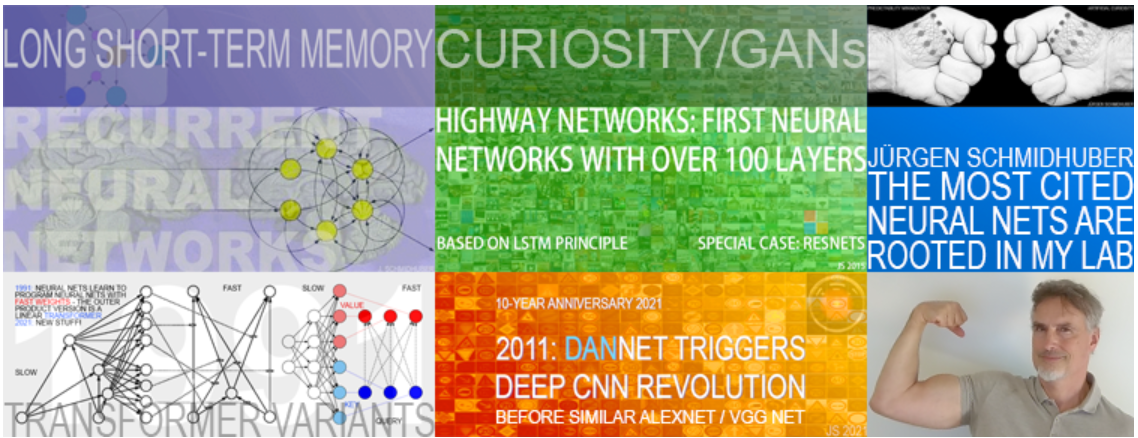
\includegraphics[height=0.5\textheight]{figures/idsia_lab.png}
\end{center}
\begin{itemize}
\item Lab with many historical contributions to deep learning and artificial intelligence\\
\link{https://people.idsia.ch/~juergen/most-cited-neural-nets.html}.
\item Affiliated with both USI and SUPSI.
\end{itemize}
\end{frame}

\begin{frame}{Your background?}
  \begin{itemize}
\item Undergraduate major?
\item Programming experience?
\item Python? C++?
\item Machine Learning? Neural networks?
\item Interest/application domain?
\end{itemize}
\vspace{2mm}
\pause
This is a course for a broad audience.\\
\vspace{2mm}
% We are also learning, and want to improve our lectures: feedback to...
But hopefully, you:
\begin{itemize}
% \item[-] be attending/have attended the lecture \textit{Machine Learning}.\\
\item[-] have interests! e.g., some vision of applications you are interested in.
\item[-] are ready to spend time for hands-on learning, e.g., debugging your code.
\end{itemize}
\end{frame}

\begin{frame}{Deep learning: impact on \\a wide range of applications}
\begin{minipage}{0.45\textwidth}
\emphbf{Image}
\begin{itemize}
\item Image classification
\item Object detection/segmentation
\item Image generation
% \item Image captioning
\item Image to image translation...
\end{itemize}
\begin{center}
    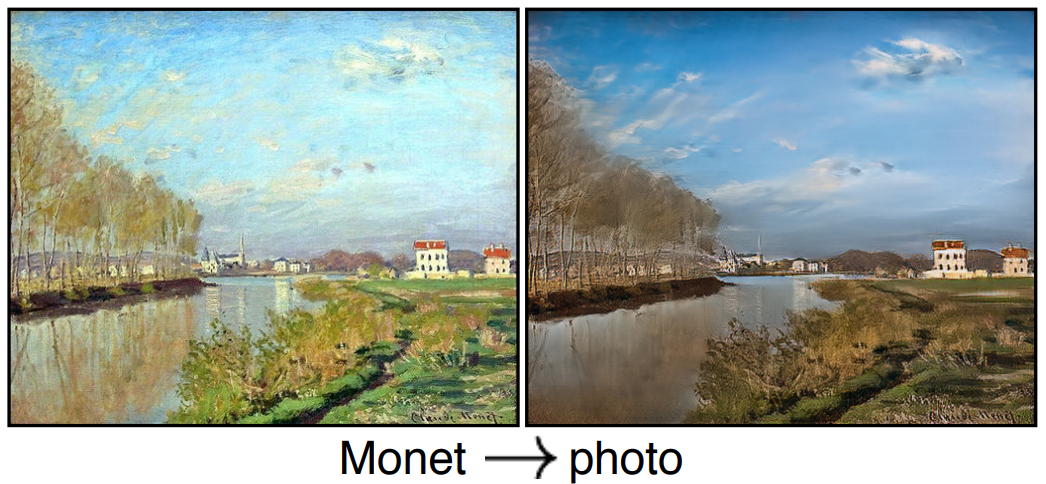
\includegraphics[height=0.3\textheight]{figures/applications/image_trans.png}
\end{center}
\vspace{-2mm}
\scriptsize{Input: Image/Paiting}\\
\scriptsize{Output: Image/Photo-realistic picture}
\end{minipage}
\begin{minipage}{0.45\textwidth}
\vspace{5mm}
\begin{center}
    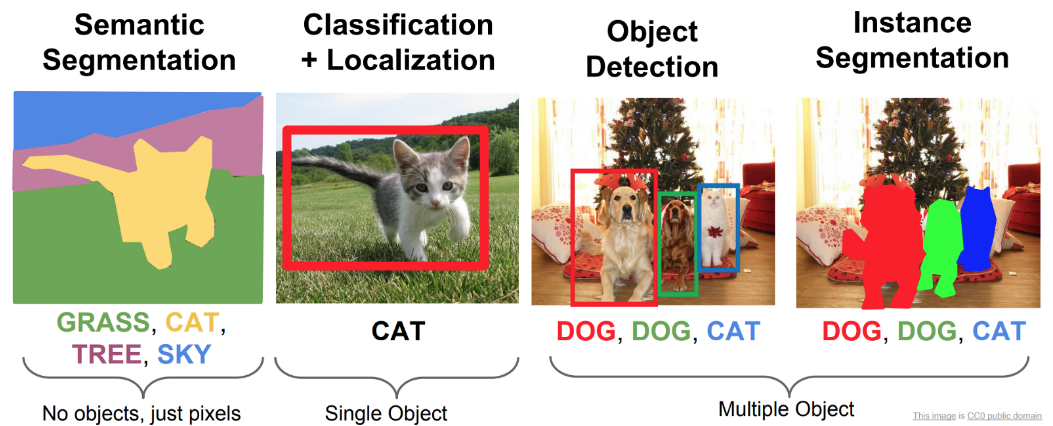
\includegraphics[height=0.35\textheight]{figures/applications/image_tasks.png}
\end{center}
% \vsp
\vspace{-2mm}
\begin{itemize}
\item Image captioning
\end{itemize}
\vspace{-5mm}
\begin{center}
    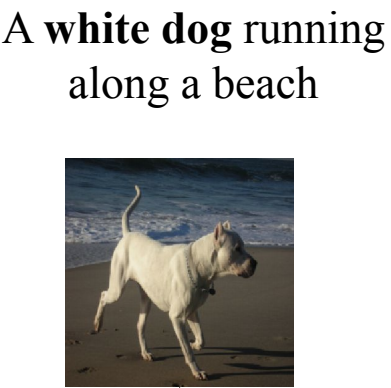
\includegraphics[height=0.3\textheight]{figures/applications/image_cap.png}
\end{center}
\vspace{-2mm}
\scriptsize{Input: Image} \\
\scriptsize{Output: Text describing the image}
 \vspace{3mm}
\end{minipage}
\hspace{5mm}
 {\footnotesize Images taken from \citem{nikolaus-etal-2019-compositional, ZhuPIE17, stanford2017}.}

%\begin{figure}
%  \begin{center}
%    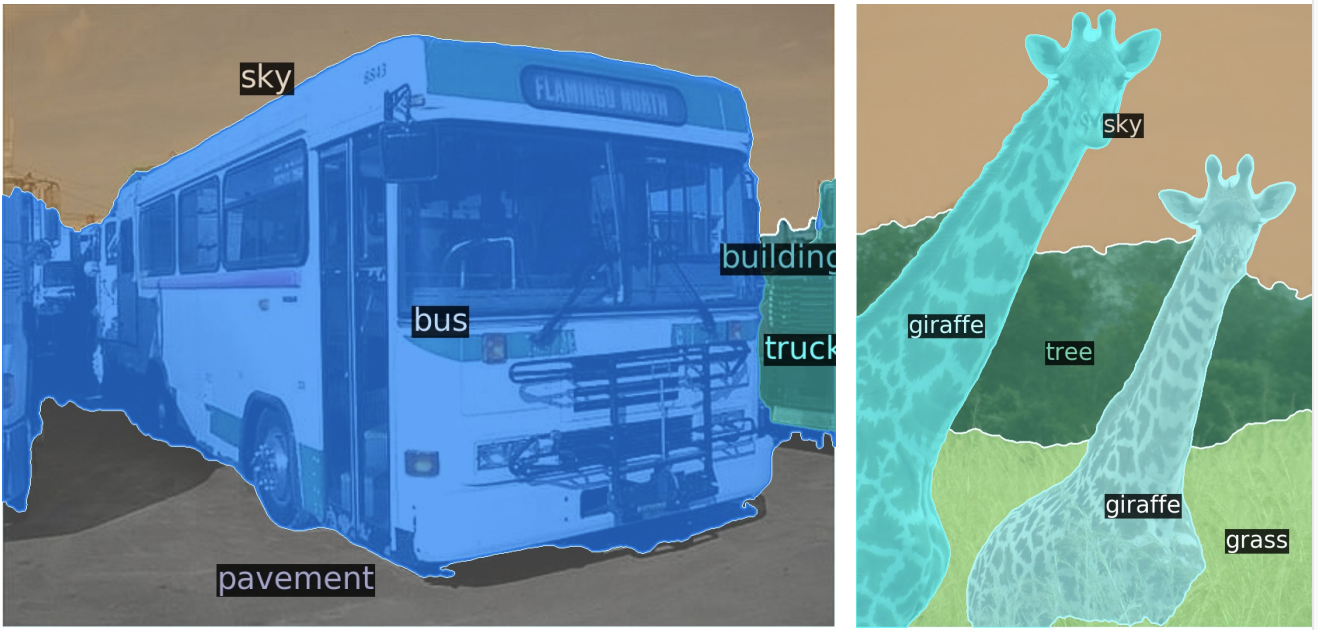
\includegraphics[height=0.5\textheight]{figures/applications/detr.png}
%  \end{center}
%\vspace{-2mm}
%\end{figure}
%    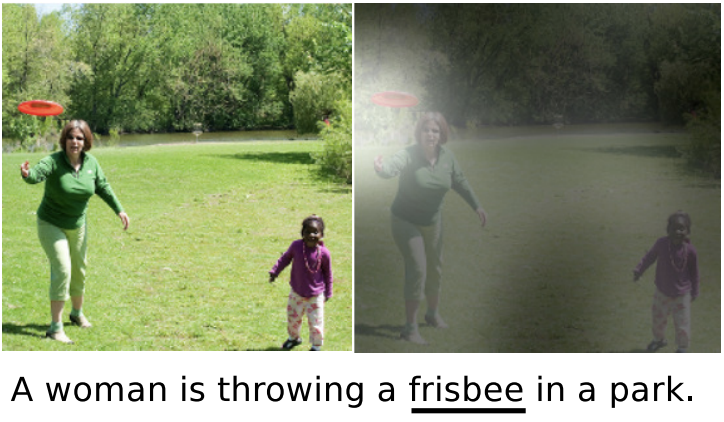
\includegraphics[height=0.3\textheight]{figures/applications/image-cap.png}
% \vspace{-2mm}
% {\small Images taken from \citem{carion2020end}.}
\end{frame}


\begin{frame}{Text to image (trending in 2022)}
%\begin{minipage}{0.45\textwidth}
\vspace{-5mm}
Imagen (Google, 2022) \link{https://imagen.research.google/}
\begin{center}
    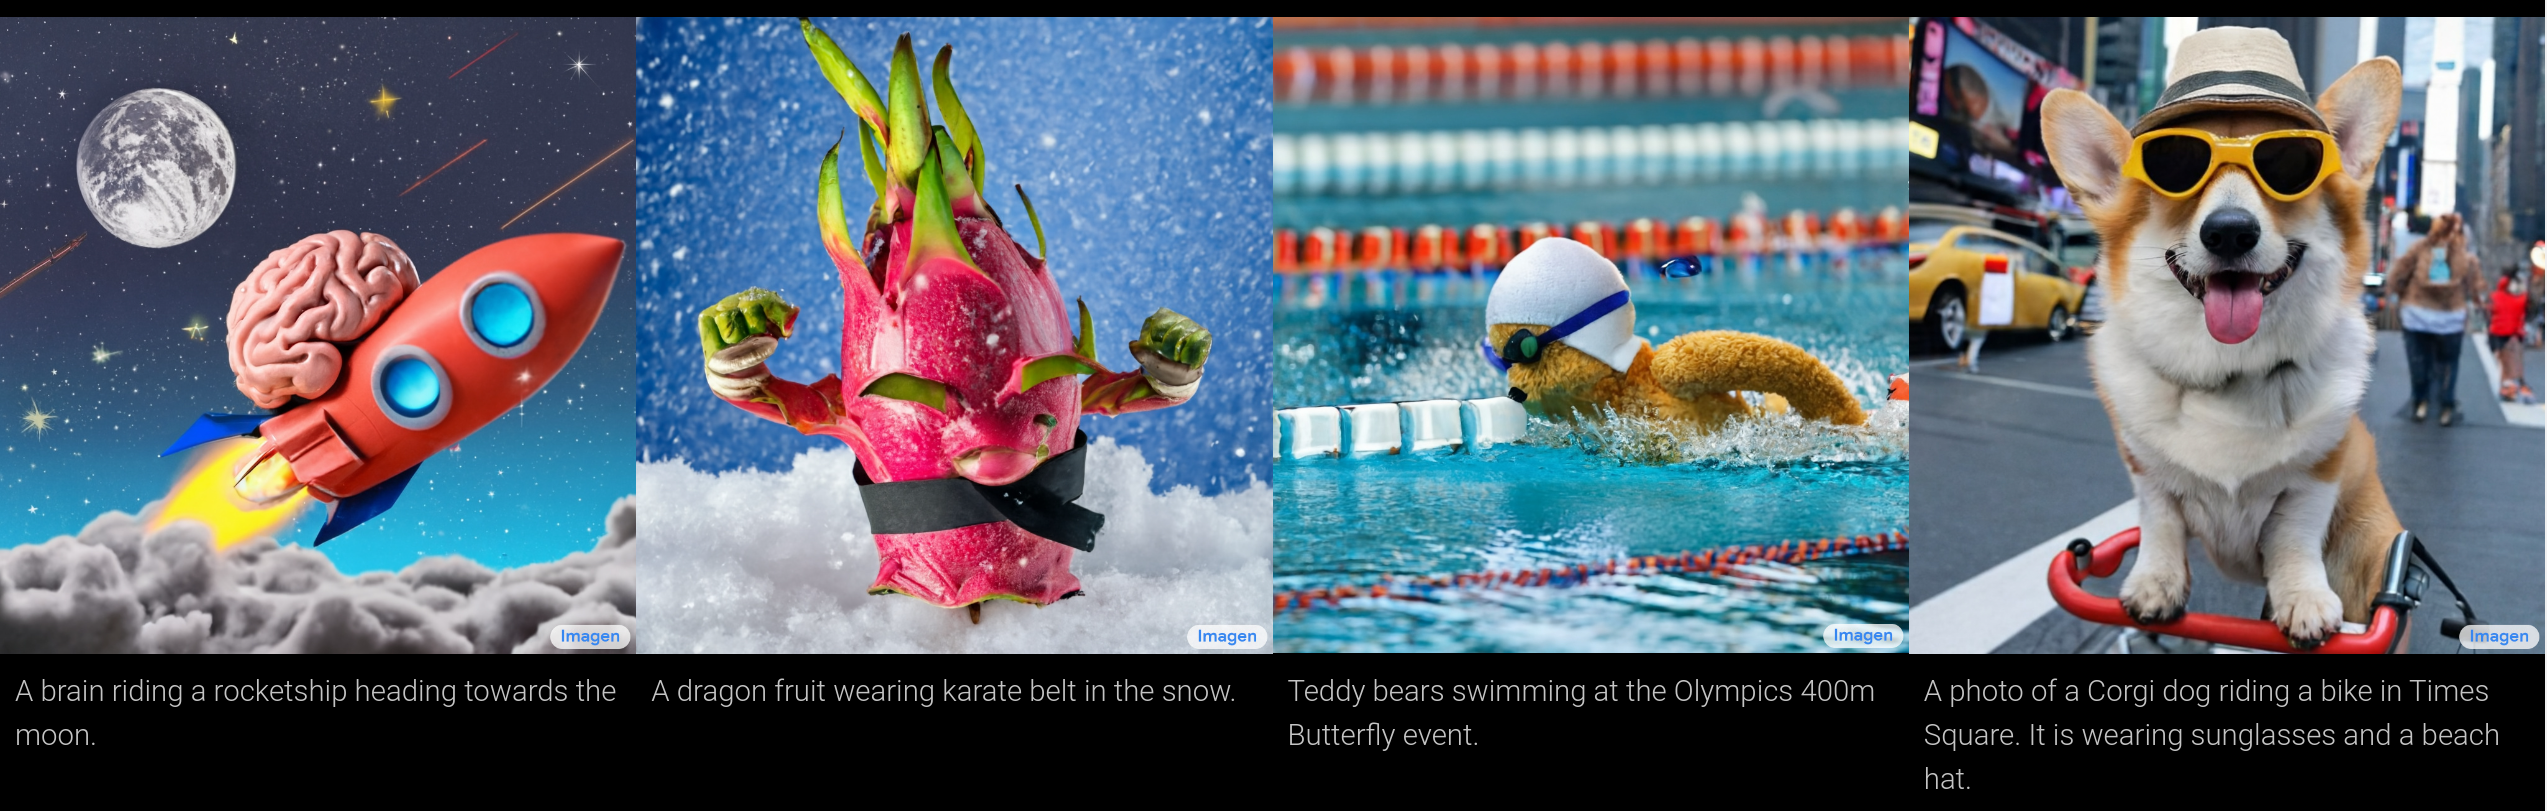
\includegraphics[height=0.5\textheight]{figures/applications/imagen_google.png}
%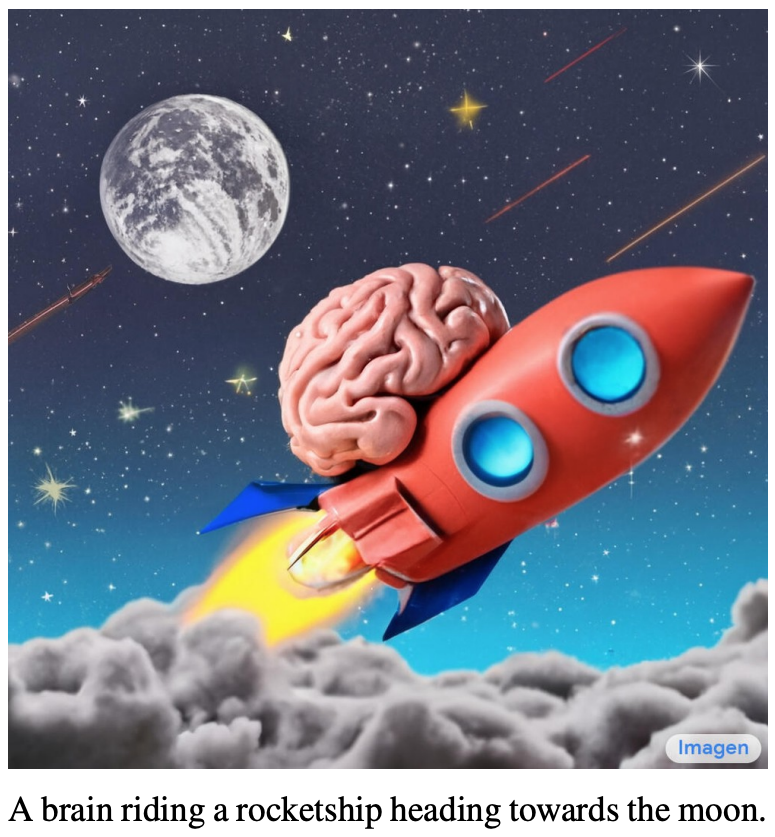
\includegraphics[height=0.5\textheight]{figures/applications/imagen_2.png}
%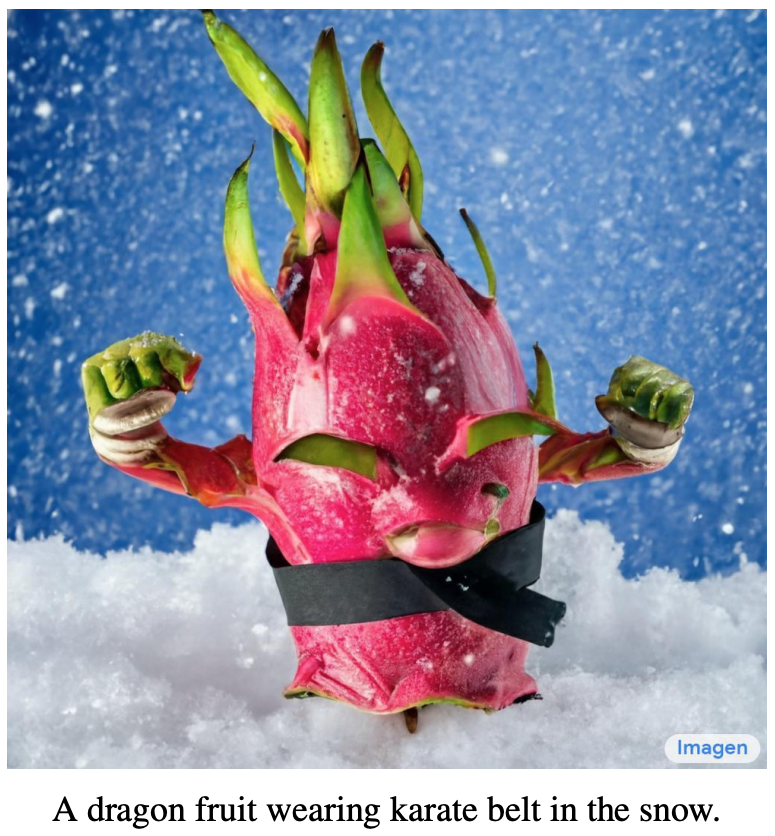
\includegraphics[height=0.5\textheight]{figures/applications/imagen_3.png}
\end{center}
%\begin{center}
%    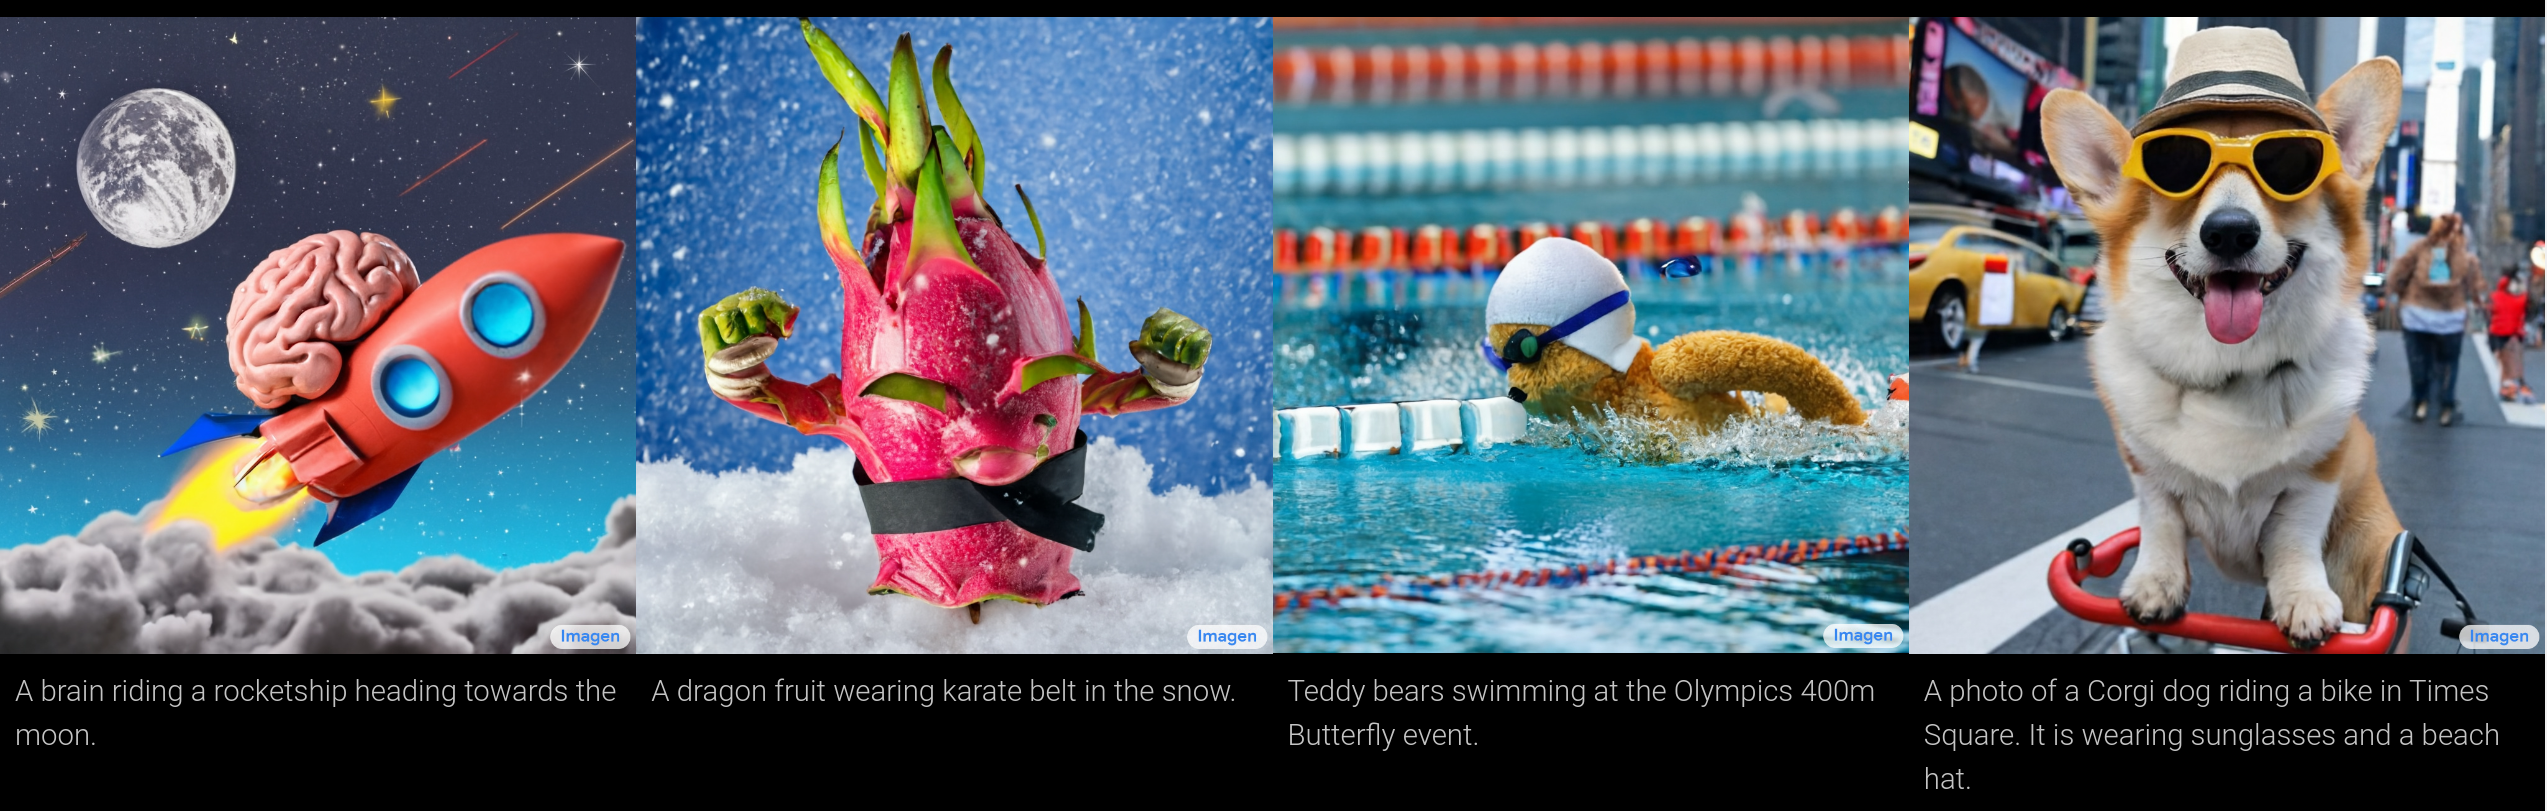
\includegraphics[height=0.5\textheight]{figures/applications/imagen_google.png}
%\end{center}
DALL-E 2 (OpenAI, 2022) \link{https://openai.com/dall-e-2/}
\begin{center}
\hspace{-20mm}
    
\includegraphics[height=0.4\textheight]{figures/applications/dalle2_1.png}
\hspace{10mm}
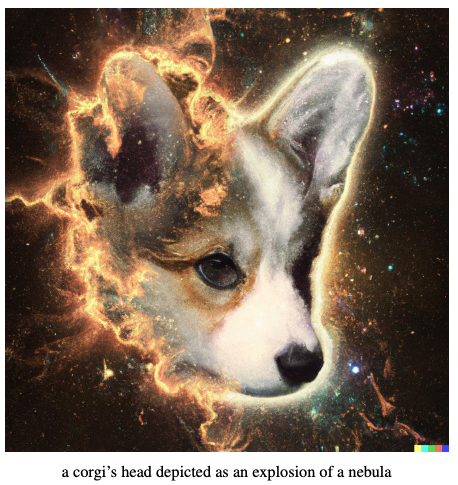
\includegraphics[height=0.4\textheight]{figures/applications/dalle2_3.png}
\hspace{10mm}
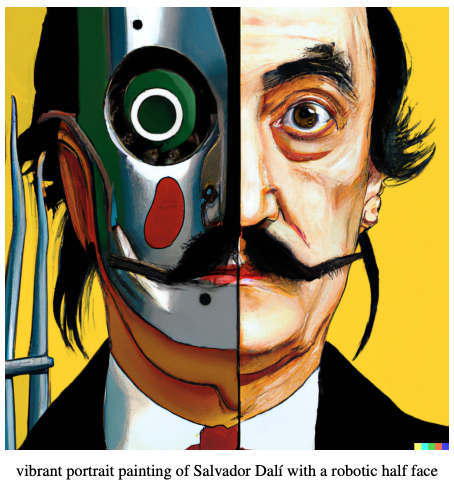
\includegraphics[height=0.4\textheight]{figures/applications/dalle2_2.png}
\end{center}
%\end{minipage}
%\begin{minipage}{0.45\textwidth}
%\vspace{5mm}
%\begin{center}
%    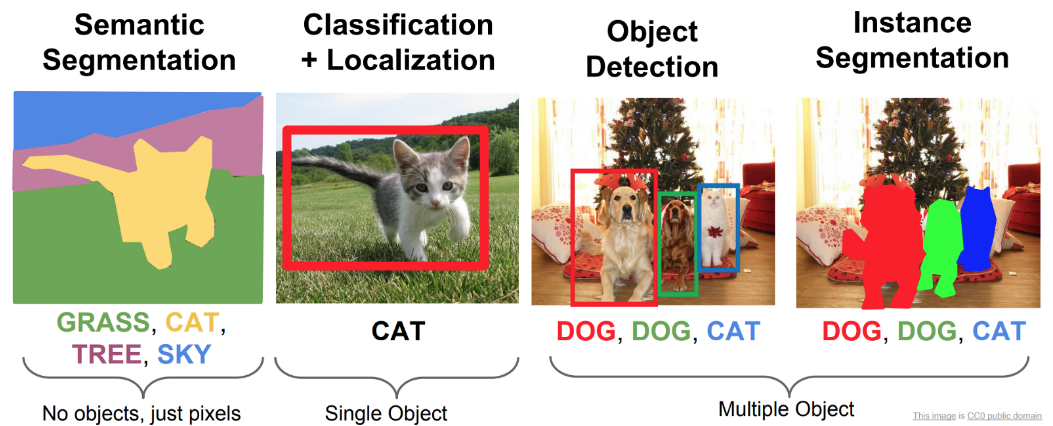
\includegraphics[height=0.35\textheight]{figures/applications/image_tasks.png}
%\end{center}
%\vsp
%\begin{center}
%    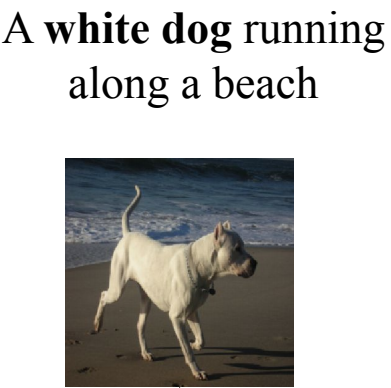
\includegraphics[height=0.3\textheight]{figures/applications/image_cap.png}
%\end{center}
%\vspace{8mm}
%\end{minipage}
%\hspace{5mm}
% {\footnotesize Images taken from \citem{nikolaus-etal-2019-compositional, ZhuPIE17, stanford2017}.}

\end{frame}

\begin{frame}{Deep learning: impact on \\wide range of applications (cont'd)}

\emphbf{Natural language \& speech}
\begin{itemize}
\item Machine translation
\item Automatic speech recognition
\item Text to speech
\item Text prediction/Language modeling
\item Text classification, generation, summarization...
\item Sentiment analysis
\item Question answering
\end{itemize}
\hspace{-8mm}
\begin{minipage}{0.2\linewidth}
  \begin{center}
    
\includegraphics[height=0.3\textheight]{figures/applications/g-translate.png}
  \end{center}
\end{minipage}
\begin{minipage}{0.35\linewidth}
  \begin{center}
    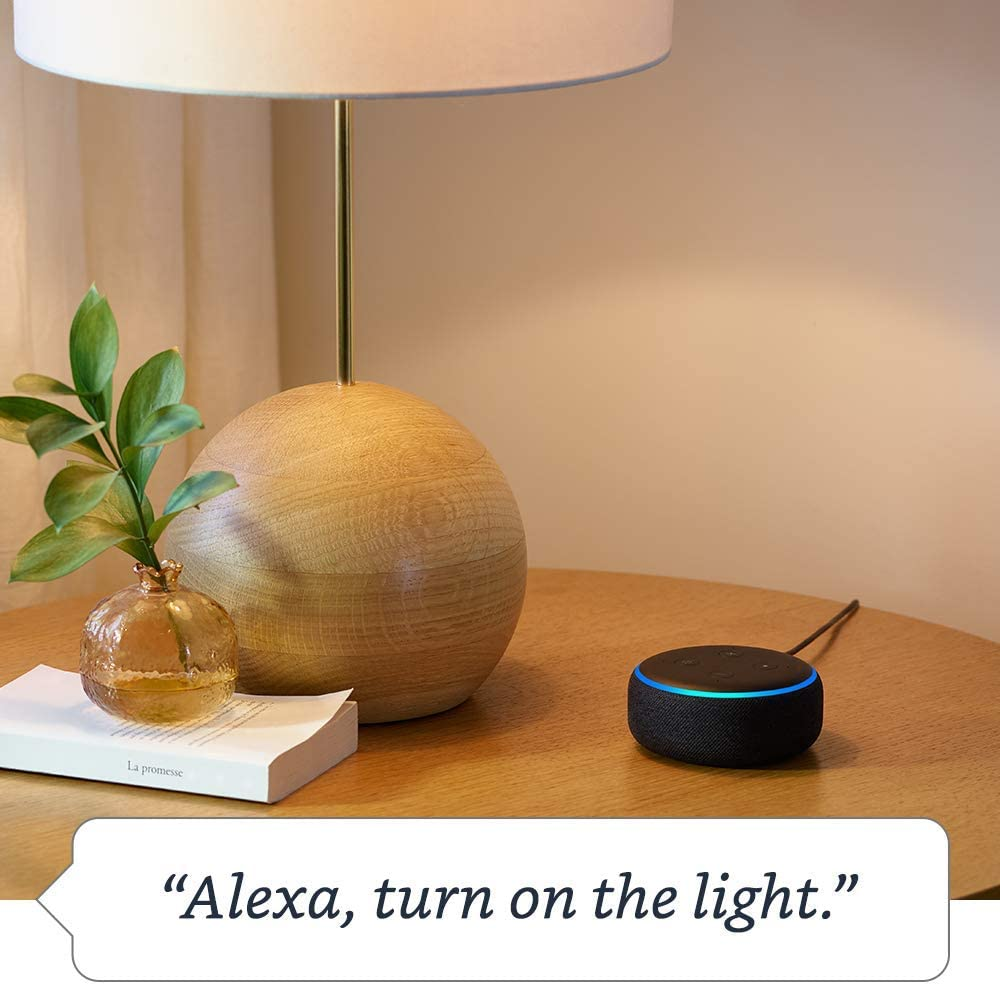
\includegraphics[height=0.4\textheight]{figures/applications/alexa.jpg}
  \end{center}
\end{minipage}
\begin{minipage}{0.35\linewidth}
  \begin{center}
    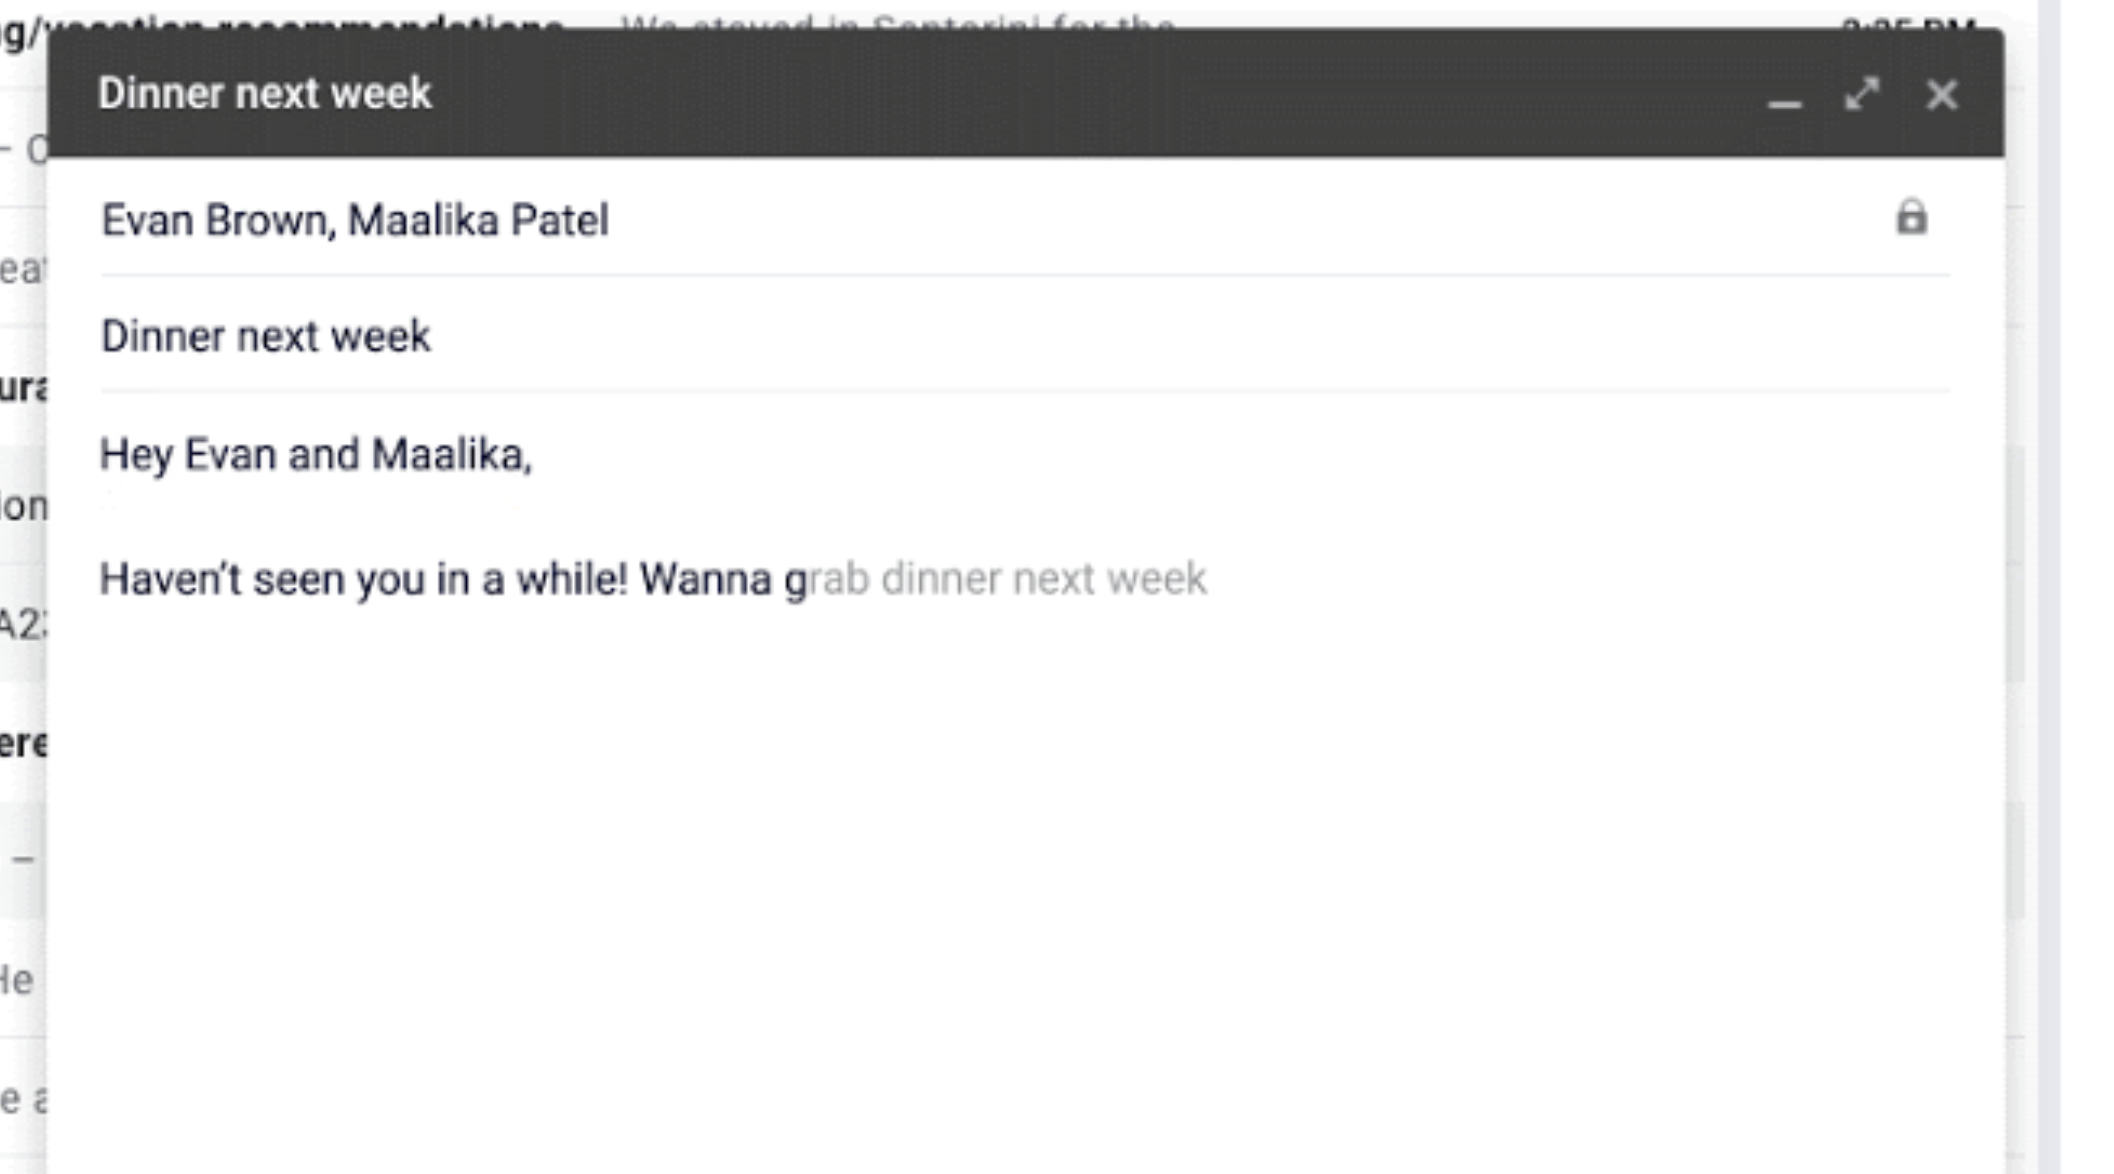
\includegraphics[height=0.5\textheight]{figures/applications/smart-compose.png}
  \end{center}
\end{minipage}
\end{frame}

\begin{frame}{Text generation (trending since 2019)}
%\begin{minipage}{0.45\textwidth}
\textbf{GPT} 2 \& 3 Language models (OpenAI, 2019/2020)
\begin{center}
    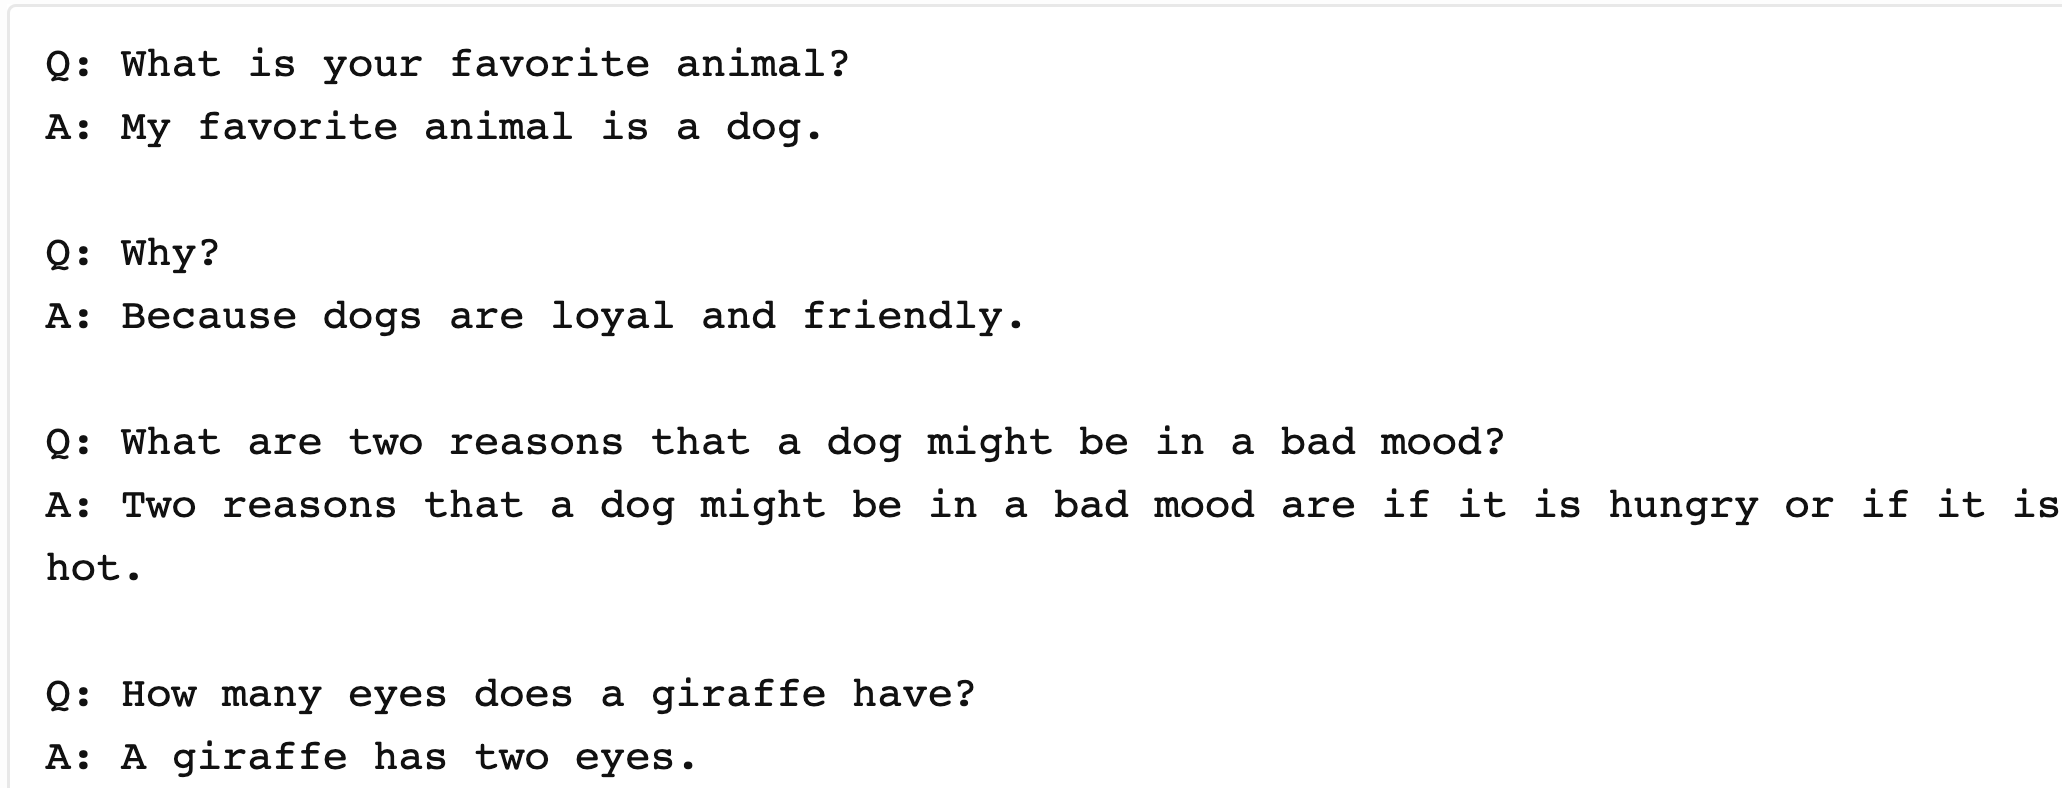
\includegraphics[height=0.6\textheight]{figures/applications/gpt_ex2.png}
\end{center}
{\small example taken from \link{https://lacker.io/ai/2020/07/06/giving-gpt-3-a-turing-test.html}}\\
Similar model applied to code generation: OpenAI Codex (2021) \\
Demo: \link{https://www.youtube.com/watch?v=SGUCcjHTmGY}

%\begin{minipage}{0.45\linewidth}
%\textbf{GPT} 2 \& 3(OpenAI, 2019/2020), text generation
%\begin{center}
%    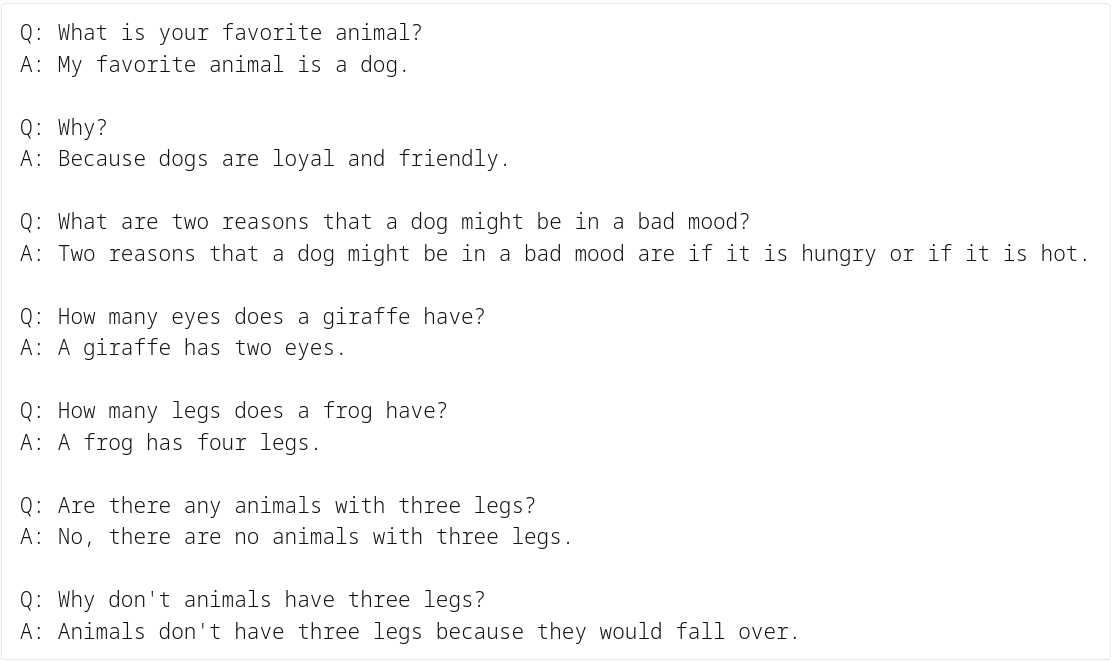
\includegraphics[height=0.5\textheight]{figures/gpt_3_output.png}
%\end{center}
%{\small example taken from \link{https://lacker.io/ai/2020/07/06/giving-gpt-3-a-turing-test.html}}
%\end{minipage}
%\vspace{3mm}
%\begin{minipage}{0.45\linewidth}
%OpenAI Codex (2021), natural language to code
%\begin{center}
%    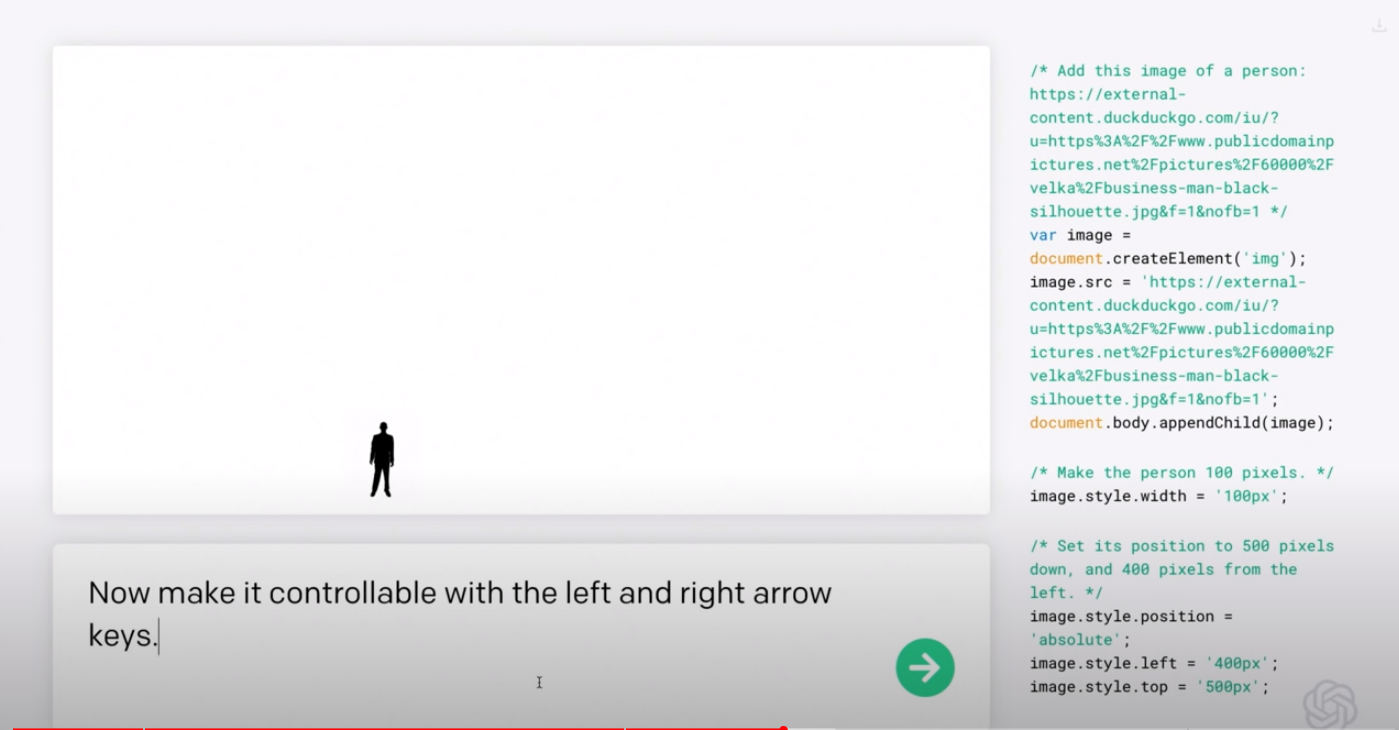
\includegraphics[height=0.3\textheight]{figures/codex_demo.png}
%\end{center}
%Demo: \link{https://www.youtube.com/watch?v=SGUCcjHTmGY}
%\end{minipage}
\end{frame}


\begin{frame}{Deep learning  applications:\\
many more domains...}
\begin{itemize}
\item Game playing (board/video games)
\item Robotics
\item Art and Music (generation)
\item Medical/pharmaceutical domain, drug discovery, chemical reaction prediction...
\item Financial engineering...
\end{itemize}
\vspace{3mm}
\begin{minipage}{0.3\linewidth}
  \begin{center}
    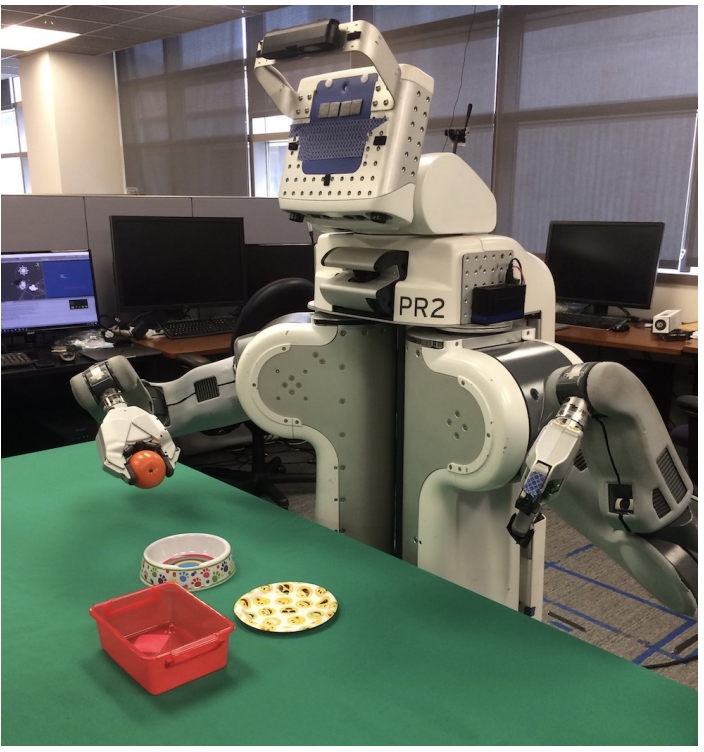
\includegraphics[height=0.5\textheight]{figures/applications/robot-manip.png}
  \end{center}
\end{minipage}
\begin{minipage}{0.25\linewidth}
  \begin{center}
    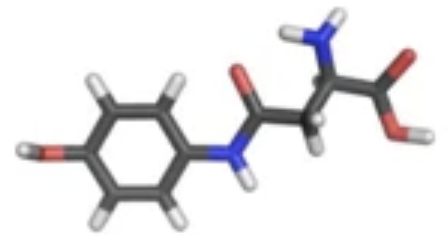
\includegraphics[height=0.2\textheight]{figures/applications/molecule.png}
  \end{center}
\end{minipage}
\begin{minipage}{0.4\linewidth}
  \begin{center}
    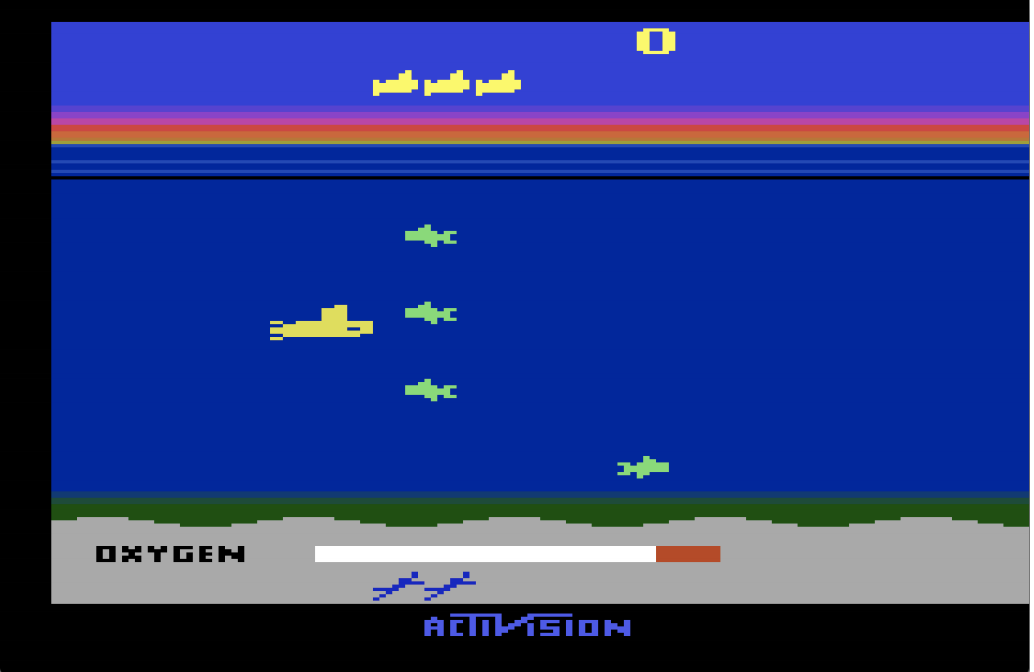
\includegraphics[height=0.4\textheight]{figures/applications/atari.png}
  \end{center}
\end{minipage}

\vspace{2mm}
{\small Figures taken from \citem{FinnYZAL17, kim2018deep, mnih-atari-2013}}
%Art/Music composition: 
%Games: video games, board games, chess, go...
%Robotics.
%OpenAI 
%Supervised learning, Reinforcement learning,...
%Also\\
%medical domain, finance...\\
\end{frame}

\begin{frame}{In this lecture...}
\vsp
\begin{itemize}
\item Unfortunately, we do not have enough time to cover everything...
\item But we'll study basic but fundamental tasks to illustrate various things that we can do with neural networks (the focus is on supervised learning).
\item Fundamental ideas are transferable to other tasks beyond in this course, and prepare you for future learning.
\item Application domains covered in the exercises:
\begin{itemize}
\item \textbf{Image classification} with feed-forward and \emphbf{convolutional neural networks}.
\item \textbf{Text generation} (and related tasks) with \emphbf{recurrent neural networks}.
\item \textbf{Mathematical problem solving} (and/or related translation-like tasks) with \emphbf{Transformers}.
\end{itemize}
\end{itemize}
%\vspace{3mm}
%\begin{minipage}{0.3\linewidth}
%  \begin{center}
%    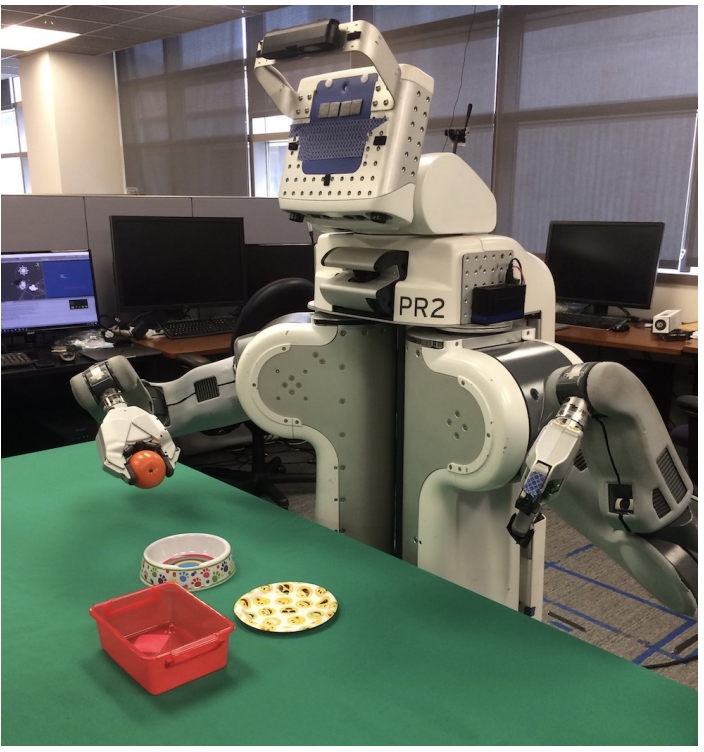
\includegraphics[height=0.5\textheight]{figures/applications/robot-manip.png}
%  \end{center}
%\end{minipage}
%\begin{minipage}{0.25\linewidth}
%  \begin{center}
%    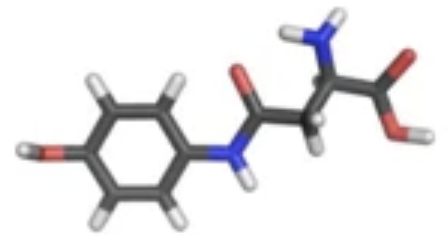
\includegraphics[height=0.2\textheight]{figures/applications/molecule.png}
%  \end{center}
%\end{minipage}
%\begin{minipage}{0.4\linewidth}
%  \begin{center}
%    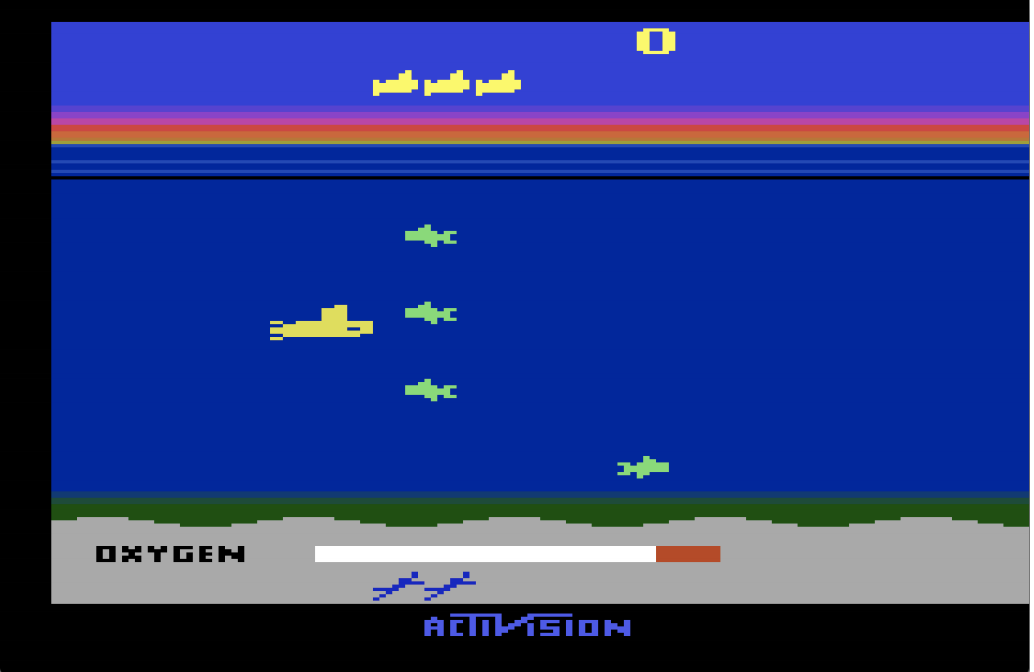
\includegraphics[height=0.4\textheight]{figures/applications/atari.png}
%  \end{center}
%\end{minipage}
%
%\vspace{2mm}
%{\small Figures taken from \citem{FinnYZAL17, kim2018deep, mnih-atari-2013}}
\end{frame}

%%%%%%%%%%%%%%%%%%%%%%%%%%%%%%%%%%%%%%%%%%%%%%%%%%%%%%%%%%%%%%%%%%%%%%%%%%

%\end{document}

%%%%%%%%%%%%%%%%%%%%%%%%%%%%%%%%%%%%%%%%%%%%%%%%%%%%%%%%%%%%%%%%%%%%%%%%%%
